\documentclass[11pt,letterpaper]{article}
\usepackage[margin=0.8in,headheight=15pt]{geometry}
\usepackage[T1]{fontenc}
\usepackage{amsmath,amssymb}
\usepackage{XCharter}
\usepackage[charter]{newtxmath}
\usepackage{microtype,graphicx,booktabs,tabularx,enumitem,xcolor,fancyhdr,titlesec,tocloft}
\usepackage{hyperref}
\usepackage[most]{tcolorbox}
\hypersetup{hidelinks,pdftitle={Aircraft Performance: Equations and Calculations Study Guide}}
\definecolor{navy}{HTML}{1F3A5F}
\definecolor{pale}{HTML}{EEF3F8}
\newtcolorbox{keyidea}{colback=pale,colframe=navy,boxrule=0.5pt,arc=1mm,breakable}
\newcommand{\val}[1]{\csname value#1\endcsname}
\newcommand{\unit}[1]{\,\mathrm{#1}}
\titleformat{\section}{\color{navy}\Large\bfseries}{\thesection}{0.65em}{}
\titlespacing*{\section}{0pt}{0pt}{14pt}
\newcommand{\topic}[1]{\clearpage\section{#1}}
\newcommand{\theorypage}[1]{\clearpage\subsection*{\color{navy}\thesection\enspace Theory: #1}}
\newcommand{\reading}[1]{{\small\color{navy}\textbf{Theory and further reading.} #1\par}\vspace{3pt}}
\renewcommand{\arraystretch}{1.16}
\setlength{\tabcolsep}{7pt}
\setlength{\abovedisplayskip}{10pt}
\setlength{\belowdisplayskip}{10pt}
\newcommand{\selfcheck}[1]{\par\textbf{Check yourself.} #1\par}
\setlength{\parindent}{0pt}
\setlength{\parskip}{6pt}
\setlist{itemsep=3pt,topsep=4pt,leftmargin=1.5em}
\setlength{\emergencystretch}{2em}
\pagestyle{fancy}\fancyhf{}
\fancyhead[L]{\small Aircraft Performance | Study Guide}
\fancyhead[R]{\small Equations and Concepts}
\fancyfoot[L]{\small V7 performance model}\fancyfoot[R]{\small\thepage}
% Calculated from V7 by make_values.py.
\expandafter\def\csname valuemass\endcsname{1,156.66}
\expandafter\def\csname valueweight\endcsname{11,342.97}
\expandafter\def\csname valuerho\endcsname{1.225012}
\expandafter\def\csname valuesound\endcsname{340.29}
\expandafter\def\csname valuevs\endcsname{27.61}
\expandafter\def\csname valuevr\endcsname{30.37}
\expandafter\def\csname valuevtwo\endcsname{33.13}
\expandafter\def\csname valueq\endcsname{564.81}
\expandafter\def\csname valuelift\endcsname{3,660.00}
\expandafter\def\csname valuedrag\endcsname{358.68}
\expandafter\def\csname valuethrust\endcsname{2,800.03}
\expandafter\def\csname valuefriction\endcsname{307.32}
\expandafter\def\csname valueaccel\endcsname{1.84}
\expandafter\def\csname valuevrkt\endcsname{59.03}
\expandafter\def\csname valuerot\endcsname{30.37}
\expandafter\def\csname valueroll\endcsname{268.61}
\expandafter\def\csname valuerolltime\endcsname{16.45}
\expandafter\def\csname valueair\endcsname{137.51}
\expandafter\def\csname valuetod\endcsname{406.11}
\expandafter\def\csname valuetodft\endcsname{1,332.40}
\expandafter\def\csname valuegrad\endcsname{15.61}
\expandafter\def\csname valueldair\endcsname{290.80}
\expandafter\def\csname valuefree\endcsname{54.99}
\expandafter\def\csname valuebrake\endcsname{107.48}
\expandafter\def\csname valueld\endcsname{453.26}
\expandafter\def\csname valueldft\endcsname{1,487.09}
\expandafter\def\csname valuevref\endcsname{31.08}
\expandafter\def\csname valuevtd\endcsname{27.49}
\expandafter\def\csname valuetempFive\endcsname{298.24}
\expandafter\def\csname valuepressFive\endcsname{84,307.11}
\expandafter\def\csname valuerhoFive\endcsname{0.9848}
\expandafter\def\csname valuesigmaFive\endcsname{0.8039}
\expandafter\def\csname valuejetvone\endcsname{126.67}
\expandafter\def\csname valuejetvr\endcsname{133.06}
\expandafter\def\csname valuejetbfl\endcsname{4,624.14}
\expandafter\def\csname valuejetgo\endcsname{4,624.14}
\expandafter\def\csname valuejetstop\endcsname{4,624.14}
\expandafter\def\csname valuejetaeo\endcsname{4,199.13}
\expandafter\def\csname valuejetfact\endcsname{4,829.00}
\expandafter\def\csname valuejettofl\endcsname{4,829.00}
\expandafter\def\csname valuekictisa\endcsname{17.64}
\expandafter\def\csname valuekictwind\endcsname{5.00}
\expandafter\def\csname valuekicttofl\endcsname{5,107.98}
\expandafter\def\csname valuekictasd\endcsname{4,896.48}
\expandafter\def\csname valuekictldr\endcsname{4,429.66}
\expandafter\def\csname valuekictmargin\endcsname{5,872.34}

\begin{document}
\begin{titlepage}
\vspace*{0.7in}{\small\color{navy}\textsc{Engineering study notes}\par}\vspace{0.35in}
{\color{navy}\Huge\bfseries Aircraft Performance\par}
\vspace{0.2in}
{\LARGE Theory, Equations\par and Worked Calculations\par}
\vspace{0.35in}
{\large A study guide for the V7 project}\par
\vspace{0.45in}
\begin{keyidea}
Learn the physical ideas first, derive the main equations, then apply them
to representative calculations and explain their limitations.
This guide covers the engineering and numerical concepts, not Python syntax.
\end{keyidea}
\vspace{0.25in}
\textbf{The calculation chain}\par
Units and conditions $\rightarrow$ density and wind $\rightarrow$ forces and speeds\\[4pt]
Ground roll and climb $\rightarrow$ takeoff or landing distance $\rightarrow$ runway comparison.
\vfill
Based on V7 equations and constants. Values are generated by
\texttt{make\_values.py}. Hand calculations may differ slightly due to rounding.\par
November 2026\par
\small Educational model; not approved flight-planning data.
\end{titlepage}
\setlength{\cftbeforesecskip}{4pt}
\renewcommand{\cftsecfont}{\small}
\renewcommand{\cftsecpagefont}{\small}
\tableofcontents
\vfill
\begin{keyidea}
\textbf{How to read the citations.} The calculations and numerical choices in this
guide follow V7. Textbook citations identify the underlying theory and suggested
reading; they do not establish that each V7 approximation appears verbatim in a
book. Chapter and section pointers for Mair \& Birdsall and Filippone were checked
against publisher contents lists. No unverified page or equation numbers are given.
\end{keyidea}
\topic{How to study this project}
For each equation, practise five things: identify the output, define every
symbol and unit, explain the physical reason for each term, substitute numbers,
and predict how the answer changes when an input changes.

\par
\begin{tabularx}{\linewidth}{@{}lX@{}}\toprule
Study block & What you should be able to do without notes\\\midrule
1. Foundations & Convert units; distinguish mass, weight, TAS and GS.\\
2. Atmosphere & Calculate ISA deviation, pressure, density and speed of sound.\\
3. Aerodynamics & Calculate lift and drag; derive stall speed from $L=W$.\\
4. Propulsion & Explain the propeller thrust cap, turbocharging, flat rating and OEI.\\
5. Flight segments & Write the accelerating and braking force balances; assemble takeoff and landing distances.\\
6. Field length & Explain the BFL crossing, AEO factor and runway margins.\\
7. Defence & Explain sensitivity, calibration, numerical integration and limitations.\\\bottomrule
\end{tabularx}

\textbf{Three kinds of equation appear here.}
\begin{itemize}
\item \textbf{Physical relations:} Newton's second law, the ideal-gas relation,
and lift/drag expressed using aerodynamic coefficients.
\item \textbf{Model approximations:} constant coefficients, fixed V-speed ratios,
constant propeller efficiency and a circular transition arc.
\item \textbf{Project factors:} wind credits, the AEO distance multiplier and
landing-distance factors. Learn how this project applies them without claiming
that it implements every certification requirement.
\end{itemize}
\begin{keyidea}
Being able to repeat a formula is the starting point. Being able to explain
why the project uses it, what is held constant, and where it can fail is the goal.
\end{keyidea}
\textbf{A useful routine:} read one section, reproduce its equations on blank
paper, do its worked calculation, then answer the check question aloud. Complete
the mixed practice set only after working through the full calculation chain.
Each added theory page belongs to the preceding topic: use it to explain why
the equations work before repeating the numerical example.

\topic{Symbols, units and signs}
\par
\begin{tabularx}{\linewidth}{@{}lXl@{}}\toprule
Symbol & Meaning & SI unit\\\midrule
$m$, $W$ & Aircraft mass; aircraft weight & kg; N\\
$T$, $D$, $L$ & Thrust, drag, lift & N\\
$\Theta$, $p$, $\rho$ & Absolute air temperature, pressure, density & K; Pa; kg/m$^3$\\
$V$, $V_{\rm GS}$ & TAS; ground speed along the runway & m/s\\
$V_w$, $V_x$ & Headwind; crosswind component & m/s or kt\\
$S$, $q$ & Reference wing area; dynamic pressure & m$^2$; Pa\\
$C_L$, $C_D$, $k$ & Lift, drag and induced-drag coefficients & dimensionless\\
$\mu$, $\theta$ & Friction coefficient; runway slope angle & dimensionless; rad\\
$\gamma$, $n$ & Climb angle; transition load factor & rad; dimensionless\\
$P$, $\eta_p$ & Shaft power; propeller efficiency & W; dimensionless\\
$a$, $a_{\rm GS}$ & Speed of sound; ground acceleration & m/s; m/s$^2$\\\bottomrule
\end{tabularx}
We use $\Theta$ for temperature to avoid confusing it with thrust $T$.
Pressure altitude $h$ is measured above the atmospheric reference; screen
height is measured above the runway.
\begin{align*}
W&=mg_0, &g_0&=9.80665\unit{m/s^2},\\
1\unit{ft}&=0.3048\unit{m}, &1\unit{kt}&=1852/3600\unit{m/s},\\
1\unit{lb}&=0.45359237\unit{kg}, &1\unit{lbf}&=4.4482216152605\unit{N},\\
1\unit{hp}&=745.69987158227\unit{W}, &\Theta[\mathrm K]&=\Theta[{}^\circ\mathrm C]+273.15.
\end{align*}
Area conversions require the \emph{square} of the length factor:
$1\unit{ft^2}=0.3048^2\unit{m^2}$. A temperature difference of $20^\circ$C equals
20 K; an absolute temperature of $20^\circ$C equals 293.15 K.

\textbf{Signs:} positive headwind opposes aircraft motion; tailwind is negative.
Positive slope is uphill in the direction of operation. Positive crosswind is
from the right. Convert degree inputs to radians before trigonometric evaluation.

\textbf{Example:} $2550\unit{lb}\times0.45359237=\val{mass}\unit{kg}$, then
$W=\val{mass}\times9.80665=\val{weight}\unit{N}$.
The number in kg is not a force.
\selfcheck{Why is multiplying pounds by $g_0$ directly wrong? Because lb must first
be converted to kg if $g_0$ is in m/s$^2$ and the required force is N.}

\topic{Atmosphere: ISA, temperature and density}
\reading{Anderson, \emph{Introduction to Flight} \cite{anderson-flight}; Filippone, Sec.~8.1 \cite{filippone}.}
The project uses a constant-lapse-rate troposphere, valid for
$0\le h\le11000\unit m$.
\begin{align*}
\Theta_{\rm std}&=288.15-0.0065h,\\
p&=101325\left(\frac{\Theta_{\rm std}}{288.15}\right)^{g_0/(0.0065R)},\\
\Theta&=\Theta_{\rm std}+\Delta\Theta_{\rm ISA},\\
\rho&=\frac{p}{R\Theta},\qquad R=287.05\unit{J/(kg\,K)},\\
\sigma&=\frac{\rho}{1.225},\qquad a=\sqrt{1.4R\Theta}.
\end{align*}
The pressure expression follows from hydrostatic balance
$dp/dh=-\rho g_0$, the ideal-gas relation and the standard temperature lapse.
An ISA deviation changes the actual temperature and density, but the pressure
at a specified \emph{pressure altitude} still follows the standard profile.

Given OAT in $^\circ$C:
\[
\Delta\Theta_{\rm ISA}=\mathrm{OAT}-(\Theta_{\rm std}-273.15).
\]
\textbf{Worked example: 5000 ft, ISA+20.}
\begin{align*}
h&=5000(0.3048)=1524\unit m,\\
\Theta_{\rm std}&=288.15-0.0065(1524)=278.244\unit K,\\
\Theta&=278.244+20=\val{tempFive}\unit K,\\
p&=\val{pressFive}\unit{Pa},\quad
\rho=\val{rhoFive}\unit{kg/m^3},\quad\sigma=\val{sigmaFive}.
\end{align*}
\begin{keyidea}
At fixed pressure altitude, hotter air has lower density because
$\rho=p/(R\Theta)$. Lower density raises the TAS needed for a given lift.
It can also reduce available power or thrust, depending on the engine model.
\end{keyidea}
\textbf{Pressure altitude versus density altitude:} pressure altitude represents
the pressure condition. Density altitude is the ISA altitude corresponding to
the actual density. This project calculates density directly; it does not need
a separate density-altitude conversion.
\selfcheck{Does ISA+20 mean the OAT is $20^\circ$C? No. It means 20 degrees above
standard temperature at that altitude.}


\theorypage{why pressure and density fall with height}
\reading{Atmosphere background: Anderson \cite{anderson-flight}; Filippone, Sec.~8.1 \cite{filippone}. The derivation below uses the V7 constants.}
\textbf{Start with a stationary layer of air.}
The pressure force from below must balance the pressure force from above and
the layer's weight. For a thin layer of thickness $dh$, the balance gives
\[
\frac{dp}{dh}=-\rho g_0.
\]
The negative sign means pressure falls as height increases. Pressure is force
per area; density is mass per volume. They are related, but they are not the
same property. Combining hydrostatic balance with the ideal-gas relation
$p=\rho R\Theta$ gives $dp/p=-g_0\,dh/(R\Theta)$.

\textbf{Where the ISA pressure exponent comes from.}
In the troposphere, assume a constant temperature lapse rate $\lambda$:
$\Theta_{\rm std}=\Theta_0-\lambda h$. Integrating from sea level to $h$ gives
\[
\ln\frac{p}{p_0}=\frac{g_0}{R\lambda}
\ln\frac{\Theta_0-\lambda h}{\Theta_0},
\qquad
p=p_0\left(\frac{\Theta_{\rm std}}{\Theta_0}\right)^{g_0/(R\lambda)}.
\]
The power law is therefore the result of hydrostatic balance, an ideal gas,
a linear temperature profile and constant gravity. It is not a universal
pressure law for every height or weather condition.

\textbf{Why a hot day changes density without changing pressure here.}
V7 takes \emph{pressure altitude} as an input: it identifies a pressure on the
standard profile. At that fixed pressure, applying ISA deviation changes
$\Theta$, so $\rho=p/(R\Theta)$ decreases as temperature increases. At the same
pressure, a change from 280 K to 300 K gives
$\rho_{300}/\rho_{280}=280/300=0.9333$: about 6.7\% less density.
This does not say pressure at a fixed geographical elevation never changes.

\textbf{Why the aircraft cares.}
Lower density reduces aerodynamic forces at a given TAS, so more TAS is needed
to generate a specified lift. It can also reduce available engine output.
The atmosphere therefore changes both the target speed and the acceleration
available to reach it. Speed of sound depends on absolute temperature through
$a=\sqrt{\gamma_{\rm air}R\Theta}$; Mach number is $V/a$.

\begin{keyidea}
\textbf{Explain aloud:} pressure altitude identifies pressure; ISA deviation
sets the temperature departure; together they determine density. Density altitude
is the altitude in ISA that would have this same density, not another name for
the input pressure altitude.
\end{keyidea}

\topic{TAS, GS and wind components}
\reading{Mair \& Birdsall, Ch.~2 \cite{mair}; Filippone, Sec.~8.2 \cite{filippone}. The wind-credit factors below describe V7.}
Aerodynamic forces depend on motion relative to air. Runway distance depends on
motion relative to the ground. For the project's along-runway model:
\[
V_{\rm TAS}=V_{\rm GS}+V_w,\qquad V_{\rm GS}=V_{\rm TAS}-V_w.
\]
At a fixed liftoff TAS, a headwind reduces the ground speed that must be reached.
For example, 70 KTAS with a 10 kt headwind corresponds to 60 kt GS; with a 10 kt
tailwind, it corresponds to 80 kt GS.

For wind \emph{from} heading $\psi_w$ and runway true heading $\psi_r$:
\begin{align*}
V_w&=V_{\rm wind}\cos(\psi_w-\psi_r),\\
V_x&=V_{\rm wind}\sin(\psi_w-\psi_r).
\end{align*}
\textbf{Example:} wind from $030^\circ$ at 20 kt, runway heading $000^\circ$:
$V_w=20\cos30^\circ=17.32$ kt and $V_x=20\sin30^\circ=10.00$ kt from the right.

The runway-analysis calculation applies:
\[
V_{w,\rm perf}=\begin{cases}0.5V_w,&V_w\ge0,\\1.5V_w,&V_w<0.\end{cases}
\]
Thus a reported 10 kt headwind becomes 5 kt, while a 10 kt tailwind becomes
$-15$ kt. These factors reduce the credited benefit and increase the penalty.
\begin{keyidea}
Use the factored wind once. A direct takeoff, landing or BFL calculation uses
the headwind supplied to it; runway analysis factors reported wind before
calling those calculations. Factoring it again would change the intended model.
\end{keyidea}
\textbf{IAS/CAS/TAS:} the project reports TAS, labelled KTAS in knots. IAS is an
instrument indication; CAS corrects instrument and position error. TAS is actual
speed through the air. Do not compare a computed KTAS directly with an AFM KCAS
schedule without the appropriate conversion.

Crosswind is reported but does not directly change this one-dimensional force
balance, nor does the project enforce an aircraft-specific crosswind limit.
\selfcheck{At brake release in a headwind, must aerodynamic lift be zero? No.
GS is zero, but TAS equals the headwind in this model.}


\theorypage{two reference frames, one aircraft}
\reading{Flight-mechanics background: Mair \& Birdsall, Ch.~2 \cite{mair}.}
\textbf{Velocity is always relative to something.}
An aerodynamic force depends on the aircraft's motion relative to the air.
Runway distance depends on its motion relative to the ground. Along the runway,
with positive $V_w$ defined as headwind,
\[
V_{\rm TAS}=V_{\rm GS}+V_w,\qquad
\frac{ds}{dt}=V_{\rm GS}=V_{\rm TAS}-V_w.
\]
The air does not need the aircraft to move over the ground before it can exert
a load. A stationary aircraft in a headwind already has airflow over it.

\textbf{Separate a force calculation from a distance calculation.}
Suppose liftoff needs 60 kt TAS and the headwind is 10 kt. The aircraft reaches
that TAS at 50 kt GS. The lift requirement is unchanged if density, weight and
configuration are unchanged, but the aircraft travels over the ground more
slowly. A 10 kt tailwind instead requires 70 kt GS for the same TAS.

For a deliberately simplified comparison, suppose each case accelerated from
rest at the same constant ground acceleration. Then $s\propto V_{\rm GS}^2$:
\[
\frac{s_{\rm head}}{s_{\rm calm}}=\left(\frac{50}{60}\right)^2=0.694,
\qquad
\frac{s_{\rm tail}}{s_{\rm calm}}=\left(\frac{70}{60}\right)^2=1.361.
\]
These ratios explain the strong sensitivity to wind. They are not V7 predictions:
in V7 the force history also changes because TAS differs at each GS.

\textbf{Why a wind component uses a cosine.}
Wind is a vector. Projecting it onto the runway gives $V_w=V\cos\Delta$;
the perpendicular projection gives crosswind $V_x=V\sin\Delta$.
The heading convention must use the direction the wind comes from consistently.
A 90-degree crosswind has no along-runway component, even though it can still
matter greatly for controllability. V7's one-dimensional force model does not
simulate lateral tyre forces or rudder control.

\textbf{A steady-wind assumption is hidden in the acceleration equation.}
If $V_w$ is constant, differentiating the velocity relation gives
$dV_{\rm TAS}/dt=dV_{\rm GS}/dt$. In a changing wind, an additional $dV_w/dt$
term appears. The project is not a wind-shear or gust-response simulation.

\begin{keyidea}
\textbf{Explain aloud:} use TAS in lift, drag and propulsion; use GS to accumulate
runway distance. A headwind does not reduce the required lift or the aircraft's
mass. It changes the relation between airspeed and ground motion.
\end{keyidea}

\topic{Lift, drag and the drag polar}
\reading{Anderson \cite{anderson-performance}; Mair \& Birdsall, Chs.~1--3 \cite{mair}.}
\begin{align*}
q&=\tfrac12\rho V_{\rm TAS}^2,\\
L&=qSC_L,\\
C_D&=C_{D_0}+kC_L^2,\\
D&=qSC_D=qS(C_{D_0}+kC_L^2).
\end{align*}
$q$ is dynamic pressure, not force. Multiplying it by area gives a force scale;
the dimensionless coefficient describes how much of that scale becomes lift or drag.
$C_{D_0}$ represents zero-lift drag in the chosen configuration. The $kC_L^2$
term represents induced drag. These coefficients are held fixed or selected by
flight segment in this project; they are not a complete aerodynamic database.

\textbf{Worked calculation.} With $\rho=1.225$, $V=40\unit{m/s}$,
$S=16.2\unit{m^2}$, $C_L=0.4$, $C_{D_0}=0.032$ and $k=0.045$:
\begin{align*}
q&=\tfrac12(1.225)(40)^2=980\unit{Pa},\\
L&=980(16.2)(0.4)=6350.4\unit N,\\
C_D&=0.032+0.045(0.4)^2=0.0392,\\
D&=980(16.2)(0.0392)=622.34\unit N.
\end{align*}
\textbf{Why induced drag is often said to fall with speed.} At \emph{fixed}
$C_L$, both lift and drag above scale with $V^2$. But in approximately level flight,
$L=W$ requires $C_L=W/(qS)$. Substituting gives:
\[
D=qSC_{D_0}+\frac{kW^2}{qS}.
\]
The first term grows with speed; the second falls with speed. Always state what
is held fixed when discussing a trend.

\textbf{Useful extension:} for a simple finite-wing approximation,
$k\approx1/(\pi e\,AR)$, where $AR=b^2/S$ and $e$ is an efficiency factor.
V7 takes $k$ as an input rather than calculating it from span and $e$.
\selfcheck{Does doubling TAS always quadruple drag? Only if density, area and
$C_D$ remain fixed. Maintaining the same lift changes $C_L$ and induced drag.}


\theorypage{why drag has two competing parts}
\reading{Anderson \cite{anderson-performance}; Mair \& Birdsall, Chs.~1--3 \cite{mair}. See also NASA's \href{https://www1.grc.nasa.gov/beginners-guide-to-aeronautics/induced-drag-coefficient/}{induced-drag explanation}.}
\textbf{What dynamic pressure means.}
The quantity $q=\rho V^2/2$ has units of pressure and provides a scale for
aerodynamic loading. Multiplying by area gives a force scale; $C_L$ and $C_D$
express how the shape, attitude and flow turn that scale into lift and drag.
The equations do not determine the coefficients themselves. Those require
data or a separate aerodynamic model.

\textbf{Why producing lift also produces drag.}
A finite wing deflects the surrounding airflow. Downwash changes the direction
of the aerodynamic force, giving a component opposing the flight direction.
A common finite-wing model is
\[
C_{D_i}=\frac{C_L^2}{\pi e\,AR}=kC_L^2,\qquad AR=\frac{b^2}{S},
\]
where $b$ is span and $e$ represents departures from an ideal spanwise loading
and other effects in the adopted polar. V7 supplies $k$ directly. Its
$C_{D_0}$ groups the modeled zero-lift drag contributions.

\textbf{The key distinction: fixed lift versus fixed lift coefficient.}
For steady level flight, set $L=W$, hence $C_L=W/(qS)$. Substituting this into
the parabolic polar gives
\[
D=qSC_{D_0}+\frac{kW^2}{qS}
=\underbrace{\tfrac12\rho S C_{D_0}V^2}_{\text{zero-lift term}}
+\underbrace{\frac{2kW^2}{\rho S V^2}}_{\text{induced term}}.
\]
At fixed weight and density, the first term rises with speed while the second
falls. Their sum has a minimum. Differentiating with respect to $q$ shows that
minimum drag occurs when the two terms are equal, giving
$C_L=\sqrt{C_{D_0}/k}$ within this idealized polar.

\textbf{Why the ground-roll model behaves differently.}
V7 holds $C_{L,\rm gnd}$ fixed during the roll. Therefore both modeled drag
terms grow with $q$, and lift grows with $q$ too. Do not use the level-flight
claim ``induced drag falls as speed rises'' for a calculation holding $C_L$
fixed. Always state what remains constant when describing a trend.

\begin{keyidea}
\textbf{Explain aloud:} the familiar U-shaped drag curve assumes lift is held
near weight. The aircraft changes $C_L$ as speed changes. A fixed-attitude
runway calculation makes a different assumption.
\end{keyidea}

\topic{Stall speed and the V-speed schedule}
\reading{Anderson \cite{anderson-performance}; Filippone, Secs.~8.2 and 9.6 \cite{filippone}. Fixed speed ratios are V7 assumptions.}
At the stall limit in the project's one-g approximation:
\[
W=L=\tfrac12\rho V_S^2SC_{L,\max}
\quad\Longrightarrow\quad
\boxed{V_S=\sqrt{\frac{2W}{\rho SC_{L,\max}}}}.
\]
Stall is associated with reaching the limiting lift coefficient, normally tied
to excessive angle of attack; the quoted stall speed depends on the conditions.
$V_{S1}$ uses takeoff flaps; $V_{S0}$ uses landing flaps here.

\par
\begin{tabularx}{\linewidth}{@{}lXl@{}}\toprule
Speed & Meaning in this model & Schedule\\\midrule
$V_R$ & Rotation speed & $1.1V_{S1}$\\
$V_2$ & Initial climb speed & $1.2V_{S1}$\\
$V_{\rm TR}$ & Transition-arc speed & $1.15V_{S1}$\\
$V_{\rm REF}$ & Landing approach speed & $1.3V_{S0}$\\
$V_{\rm TD}$ & Touchdown speed & $1.15V_{S0}$\\
$V_1$ & Engine-failure/decision-speed trial & Solved from go/stop distances\\\bottomrule
\end{tabularx}

\textbf{Scaling you should know:}
\[
V_S\propto\sqrt W,\qquad V_S\propto\rho^{-1/2},\qquad
V_S\propto C_{L,\max}^{-1/2}.
\]
Increasing weight by 10\% raises stall speed by $\sqrt{1.10}-1=4.88\%$.
Reducing density to 80\% raises stall TAS by $1/\sqrt{0.8}-1=11.80\%$.
Neither percentage is the same as the eventual takeoff-distance change.

\textbf{C172 example:} using $W=\val{weight}\unit N$, $S=16.2\unit{m^2}$,
$C_{L,\max,TO}=1.5$ and the model's sea-level density:
\[
V_{S1}=\val{vs}\unit{m/s},\quad V_R=\val{vr}\unit{m/s}
=\val{vrkt}\unit{KTAS},\quad V_2=\val{vtwo}\unit{m/s}.
\]
\begin{keyidea}
The fixed multipliers are project assumptions, not a universal certified
V-speed schedule. The model does not independently calculate VMCG, VMU or VLOF.
\end{keyidea}
\selfcheck{Does a 20\% increase in $C_{L,\max}$ reduce stall speed by 20\%? No:
the speed factor is $1/\sqrt{1.2}=0.9129$, a reduction of 8.71\%.}


\theorypage{stall is a lift limit, not an arbitrary speed}
\reading{Anderson \cite{anderson-performance,anderson-flight}; Filippone, Sec.~8.2 \cite{filippone}.}
\textbf{Begin with angle of attack.}
Angle of attack is the angle between the wing's reference chord and the relative
airflow. Increasing it generally raises $C_L$ over a useful range. Beyond a
critical region, substantial flow separation limits the lift coefficient.
The peak value is represented by $C_{L,\max}$ for a given configuration.
Stall is therefore tied to the aerodynamic state, not one universal indicated
or true airspeed.

\textbf{Derive the speed from the required lift.}
For unaccelerated level flight, or the project's simplified lift-off threshold,
require $L=W$ and set $C_L=C_{L,\max}$:
\[
W=\tfrac12\rho V_S^2 S C_{L,\max}
\quad\Longrightarrow\quad
V_S=\sqrt{\frac{2W}{\rho S C_{L,\max}}}.
\]
This is TAS when local density is used. It assumes a known maximum lift
coefficient and ignores detailed ground effect, transient pitch dynamics and
configuration changes during rotation.

\textbf{Use ratios to understand the square root.}
With everything else fixed, 10\% more weight raises stall speed by
$\sqrt{1.10}-1=4.88\%$. A 20\% reduction in density raises it by
$1/\sqrt{0.8}-1=11.8\%$. Increasing $C_{L,\max}$ helps reduce stall speed,
but a high-lift configuration can also add drag. A lower liftoff speed alone
does not prove better climb performance.

\textbf{What happens when the aircraft must produce more than its weight?}
Define load factor $n=L/W$. For the same density and configuration,
\[
V_{S,n}=\sqrt{\frac{2nW}{\rho S C_{L,\max}}}=V_{S,1}\sqrt n.
\]
For example, $n=1.2$ raises the corresponding stall speed by about 9.54\%.
This is a background relationship, not an additional V-speed rule implemented
by V7. It explains why a manoeuvring aircraft can stall at a higher speed.

\textbf{Why scheduled speeds include margins.}
VR, V2 and VREF serve different flight phases. Ratios to a reference stall
speed provide a simple schedule for a study model. A real schedule must also
respect control, handling and other aircraft-specific constraints. V7's ratios
are inputs to an approximation; the lift equation alone does not prescribe them.
\begin{keyidea}
\textbf{Explain aloud:} stall speed is the speed at which the demanded lift
reaches the configuration's available maximum lift coefficient under the
stated assumptions.
\end{keyidea}

\topic{Propeller power, thrust and turbocharging}
\reading{Mair \& Birdsall, Ch.~5 \cite{mair}; Filippone, Ch.~6 \cite{filippone}; Gudmundsson \cite{gudmundsson}. The piecewise thrust cap is the project model.}
Power and thrust are different quantities. Useful propulsive power is $TV$;
if propeller efficiency is $\eta_p$, then $TV=\eta_pP$ and $T=\eta_pP/V$.
V7 limits this relation at low speed:
\[
T_{\rm prop}=\min\left(\sigma_P T_{\rm SLS},
\frac{\eta_p\sigma_PP_{\max}}{\max(V,1\unit{m/s})}\right)f_e.
\]
The static-thrust cap prevents the $1/V$ relation predicting infinite thrust
at rest. $T_{\rm SLS}$ and $P_{\max}$ are totals for all engines.
\[
\sigma_P=\begin{cases}
\sigma(h,\Delta\Theta),&\text{normally aspirated},\\
1,&\text{turbocharged and }h\le h_{\rm crit},\\
\sigma(h,\Delta\Theta)/\sigma(h_{\rm crit},\Delta\Theta),&h>h_{\rm crit}.
\end{cases}
\]
Below critical altitude, the turbocharged model retains rated power. Above it,
power falls with the density ratio relative to the critical-altitude condition.
This is a simplified engine model: temperature penalties below critical altitude,
mixture control and detailed propeller efficiency maps are not included.

\textbf{Example:} at $V=40\unit{m/s}$, $P=134000\unit W$ and $\eta_p=0.65$,
$\eta_pP/V=2177.5\unit N$. If static thrust is 2800 N, the power expression limits
thrust to 2177.5 N. At 10 m/s it predicts 8710 N, so the static cap limits it to
2800 N. This illustration uses $\sigma_P=1$ and all engines.

\textbf{OEI thrust fraction:}
\[
f_e=\frac{N_{\rm op}}{N_e},\qquad N_{\rm op}=N_e-1\quad\text{for OEI}.
\]
A twin therefore retains half its modelled total thrust. This assumes equal
engines and omits additional failed-engine drag.
\selfcheck{Does losing half the thrust halve climb performance? No. Climb depends
on excess thrust $T-D$. If drag was already large, the remaining excess can be
much less than half or can become negative.}

\topic{Jet thrust, Mach number and flat rating}
\reading{Filippone, Secs.~5.2--5.3 \cite{filippone}; Mair \& Birdsall, Ch.~5 \cite{mair}. V7 uses its own simplified thrust fit.}
V7 uses this approximate turbofan thrust law:
\begin{align*}
\Delta\Theta_{\rm excess}&=\max(\Delta\Theta_{\rm ISA}-\Delta\Theta_{\rm flat},0),\\
\sigma_{\rm eff}&=\sigma(h,\Delta\Theta_{\rm excess}),\\
M&=V/a(h,\Delta\Theta_{\rm ISA}),\\
T_{\rm jet}&=T_{\rm SLS}\sigma_{\rm eff}^{0.7}(1-k_{\rm lapse}M)f_e.
\end{align*}
The Challenger uses $\Delta\Theta_{\rm flat}=15^\circ$C and
$k_{\rm lapse}=0.90$. Altitude still affects $\sigma_{\rm eff}$ below the
flat-rating temperature. The actual temperature is used for speed of sound.

\textbf{Flat rating in this implementation:}
\begin{itemize}
\item ISA+10 and ISA+15 both give zero excess temperature.
\item ISA+25 gives an excess of $10^\circ$C, reducing effective density and thrust.
\item At zero TAS, $M=0$: the Mach multiplier is one.
\item At nonzero TAS, temperature can still affect thrust through $a$ and $M$,
even below the flat-rating limit. Thus ``perfectly constant thrust below ISA+15''
is not exact for this model at every speed.
\end{itemize}
\textbf{Illustration:} take $T_{\rm SLS}=65000\unit N$, $\sigma_{\rm eff}=1$,
$V=70\unit{m/s}$ and $a=340\unit{m/s}$. Then $M=0.20588$ and
$T=65000[1-0.9(0.20588)]=52955.9\unit N$ AEO; OEI gives 26477.9 N for a twin.

\textbf{Reverse thrust during braking:}
\[
T_{\rm rev}=\begin{cases}r_{\rm rev}T_{\rm SLS},&\text{enabled and TAS}>60\unit{kt},\\
0,&\text{otherwise}.\end{cases}
\]
The code uses TAS for the cutoff and a constant fraction of SLS thrust above it.
This is an approximation, not a detailed reverser schedule. The propeller class
returns zero reverse thrust.
\selfcheck{Why is this not a full engine model? Its density exponent, Mach lapse,
flat rating and reverser fraction approximate behaviour without an engine deck.}


\theorypage{power and thrust describe different things}
\reading{Mair \& Birdsall, Ch.~5 \cite{mair}; Filippone, Chs.~5--6 \cite{filippone}; Gudmundsson \cite{gudmundsson}.}
\textbf{Thrust is a force; power is a rate of doing work.}
Moving through distance $ds$ with force $T$ aligned with the motion does work
$dE=T\,ds$. Dividing by time gives useful propulsive power $P_{\rm useful}=TV$.
For a propeller receiving shaft power $P$, use efficiency $\eta_p$ to write
\[
TV=\eta_p P,\qquad T=\frac{\eta_p P}{V}.
\]
At approximately constant power and efficiency, thrust decreases as speed rises.
This helps explain why acceleration can weaken toward the end of a takeoff roll.
It does not imply thrust becomes physically infinite at rest.

\textbf{Why static thrust needs separate treatment.}
The expression above assumes an efficiency appropriate to the operating point.
At $V=0$, useful aircraft translational power $TV$ is zero even while a propeller
produces finite thrust and puts energy into the air. Treating $\eta_p$ as a
nonzero constant down to zero speed breaks the model. V7 avoids the singularity
with a lower speed bound and a static-thrust cap. The cap is a practical model
choice, not a derivation of propeller aerodynamics.

\textbf{Why density affects engine output.}
A normally aspirated piston engine ingests less air mass in thinner air.
Less available oxygen constrains the fuel that can be burned effectively,
so available power generally falls. V7 approximates the loss with a density
ratio. Turbocharging can maintain intake conditions over part of the altitude
range; the project's critical altitude marks where its simplified power-holding
assumption ends. Real limits depend on the engine and its controls.

\textbf{A jet needs a different approximation.}
Jet thrust depends on mass flow, exhaust momentum, pressure forces and operating
conditions. A power-divided-by-speed model is not interchangeable with a jet
engine model. V7 instead uses a density/Mach fit. Flat rating represents a
control or rating limit: cool-day capability can exceed the permitted rating,
so a rise in temperature need not immediately reduce rated thrust. It does not
remove every altitude or speed effect.

\begin{keyidea}
\textbf{Explain aloud:} OEI removes an engine's contribution to total thrust,
but climb depends on the thrust remaining \emph{after drag}. Losing half the
thrust can remove much more than half the excess thrust.
\end{keyidea}

\topic{Ground roll: Newton's second law}
\reading{Mair \& Birdsall, Ch.~6 \cite{mair}; Filippone, Secs.~9.2.1--9.2.2 \cite{filippone}.}
Let $s$ be distance along the runway and $\theta$ the runway slope:
\[
\theta=\arctan(\mathrm{slope}_{\%}/100),\qquad N=\max(W-L,0).
\]
$N$ is the project's approximate wheel load. A more complete inclined-runway
balance would use $W\cos\theta-L$; V7 uses $W-L$ for the small-slope approximation.

\textbf{Acceleration:}
\[
\boxed{\frac{dV_{\rm GS}}{dt}=\frac{T-D-\mu_{\rm roll}N-W\sin\theta}{m}},
\qquad \frac{ds}{dt}=V_{\rm GS}.
\]
Thrust accelerates the aircraft; drag and rolling friction oppose it. An uphill
slope subtracts available force. Lift reduces wheel load and therefore rolling
friction. The $\max$ prevents a negative friction force if computed lift exceeds weight.

\textbf{Braking:}
\[
\boxed{\frac{dV_{\rm GS}}{dt}=-\frac{D+\mu_{\rm brake}N+T_{\rm rev}+W\sin\theta}{m}}.
\]
An uphill slope assists stopping. A downhill slope has negative $\sin\theta$
and weakens deceleration. Jet ground spoilers set braking $C_L=0$, which
increases wheel load and braking force in this model. Idle thrust is zero.

\textbf{Wet runway:} $\mu_{\rm brake,wet}=0.5\mu_{\rm brake,dry}$.
This is a fixed V7 approximation, not a universal tyre--runway law.
It affects braking, not the project's rolling coefficient. Therefore wetness
alone does not change its AEO takeoff calculation, but does change accelerate-stop.

\textbf{Illustration:} $m=1200$ kg, $T=2500$ N, $D=500$ N,
$L=4000$ N, $\mu_{\rm roll}=0.04$, level runway:
\[
W=11767.98\unit N,\quad F_{\rm roll}=0.04(11767.98-4000)=310.72\unit N,
\]
\[
a_{\rm GS}=(2500-500-310.72)/1200=1.4077\unit{m/s^2}.
\]
A 1\% uphill slope adds about 117.67 N of resistance, reducing acceleration by
about $0.0981\unit{m/s^2}$.
\selfcheck{Why does raising lift help rolling but hurt braking? Both use wheel load:
less load reduces unwanted rolling resistance but also reduces useful tyre braking.}


\theorypage{wheel load, slope and energy}
\reading{Ground-performance background: Mair \& Birdsall, Ch.~6 \cite{mair}; Ojha \cite{ojha}.}
\textbf{Resolve forces in the direction of travel.}
On an uphill runway, gravity has a component $W\sin\theta$ opposing motion.
For small slopes, $\theta\approx\tan\theta=\text{slope percent}/100$.
Thus a 1\% uphill slope adds approximately $0.01W$ of resistance. Dividing by
mass gives an acceleration penalty close to $0.01g_0$, independent of mass
for that isolated gravity term.

\textbf{Why wheel load is not always equal to weight.}
On a level runway, vertical force balance gives $N+L\approx W$ while the gear
remains on the ground. This leads to $N\approx W-L$. For an inclined runway,
a more detailed normal balance would involve $W\cos\theta$ and the directions
of lift and thrust. V7 retains $N=\max(W-L,0)$ as a small-slope approximation.
The maximum prevents unphysical negative tyre load; it does not model liftoff
or suspension dynamics by itself.

Rolling resistance and braking both depend on tyre load in this model:
$F_{\rm roll}=\mu_{\rm roll}N$ and $F_{\rm brake}=\mu_{\rm brake}N$.
Lift reduces unwanted rolling resistance during acceleration. During braking,
the same reduction in tyre load reduces useful braking force. Spoilers help
transfer load back to the wheels. Real friction also depends on speed, slip,
tyres and runway condition; a single coefficient suppresses these details.

\textbf{An energy view of the same calculation.}
For constant mass in the ground frame, Newton's law gives
\[
\frac{d}{dt}\left(\tfrac12 mV_{\rm GS}^2\right)
=F_{\rm net}V_{\rm GS},\qquad
\Delta\left(\tfrac12mV_{\rm GS}^2\right)=\int F_{\rm net}\,ds.
\]
With constant braking force $F_b$, stopping from speed $V_0$ takes
$s=mV_0^2/(2F_b)$. If $F_b=\mu mg_0$ and all other effects are ignored,
$s=V_0^2/(2\mu g_0)$. Mass cancels in this special case. That does not mean
weight is irrelevant in V7: scheduled speeds, lift, propulsion and force
histories change with the operating case.

\begin{keyidea}
\textbf{Explain aloud:} twice the stopping speed requires four times the
kinetic-energy removal. Runway length can grow rapidly even when speed changes
seem modest. The actual brake-energy share also depends on aerodynamic drag,
reverse thrust and other forces.
\end{keyidea}

\topic{Numerical integration: why distance is not one division}
\reading{Filippone, Sec.~9.3 \cite{filippone}, for the performance problem; SciPy documentation \cite{scipy-ivp} for the solver used by V7.}
The ground-roll forces vary with TAS. Lift and drag change with $V^2$, thrust can
change with speed, and wheel load changes with lift. Acceleration therefore is
not generally constant.

\textbf{Constant-acceleration check only:}
\[
s-s_0=\frac{V_{{\rm GS},f}^2-V_{{\rm GS},0}^2}{2a_{\rm GS}}.
\]
This is useful for an order-of-magnitude check, not as a substitute for the
project's integration. At constant deceleration magnitude $b$, stopping distance
is $V_{{\rm GS},0}^2/(2b)$. A 10\% higher initial GS would then require 21\% more
stopping distance, if $b$ really stayed constant.

\textbf{A hand-calculation stepping method:}
\begin{align*}
V_{{\rm GS},i+1}&\approx V_{{\rm GS},i}+a_i\Delta t,\\
s_{i+1}&\approx s_i+V_{{\rm GS},i}\Delta t.
\end{align*}
These are forward-Euler updates, included to explain integration. They are not
the RK45 algorithm used by V7. For $V_{{\rm GS},i}=20$ m/s, $a_i=2$ m/s$^2$ and
$\Delta t=0.5$ s, the new speed is 21 m/s and Euler adds 10 m of distance.
Exact constant-acceleration motion would add 10.25 m over that interval.

\textbf{What V7 actually does:} adaptive RK45 advances the state $[s,V_{\rm GS}]$,
using several derivative evaluations to estimate local error and choose a step.
The maximum step is 0.5 s, not a fixed step. The maximum interval is 300 s.
\begin{align*}
g_{\rm accel}&=V_{\rm GS}+V_w-V_{\rm target},\\
g_{\rm stop}&=V_{\rm GS}-0.1.
\end{align*}
Acceleration stops at an upward crossing of the target TAS. Braking stops at a
downward crossing of 0.1 m/s GS, the practical stopping threshold.
\begin{keyidea}
Numerical precision is not physical accuracy. Small integration error does not
correct an inaccurate drag coefficient, thrust estimate or runway assumption.
\end{keyidea}
\selfcheck{What would a step-size study show? Whether the numerical result is stable
as the step limit is reduced. It would not validate the aircraft model itself.}


\theorypage{integration, events and numerical error}
\reading{Performance equations: Filippone, Sec.~9.3 \cite{filippone}. V7's solver interface: SciPy \cite{scipy-ivp,scipy-brent}.}
\textbf{The state contains what we need to advance.}
For the roll, use $\mathbf y=[s,V_{\rm GS}]^{\mathsf T}$. The force calculation
returns the derivatives $\mathbf f=[V_{\rm GS},F_{\rm net}/m]^{\mathsf T}$.
Integration repeatedly estimates how these changing derivatives accumulate.
The initial conditions are as important as the force equation: accelerating
from rest is a different problem from continuing after an engine failure.

\textbf{Why evaluating the acceleration once is not enough.}
An Euler step uses the derivative only at the start. As speed rises within the
step, aerodynamic forces and sometimes thrust change. Using the old derivative
throughout introduces truncation error. Runge--Kutta methods sample intermediate
states to better represent that variation.

\textbf{Connection to the Fortran ground-roll demonstration.}
For step $\Delta t$, classical RK4 uses
\begin{align*}
\mathbf k_1&=\mathbf f(\mathbf y_i),\\
\mathbf k_2&=\mathbf f(\mathbf y_i+\tfrac12\Delta t\mathbf k_1),\\
\mathbf k_3&=\mathbf f(\mathbf y_i+\tfrac12\Delta t\mathbf k_2),\\
\mathbf k_4&=\mathbf f(\mathbf y_i+\Delta t\mathbf k_3),\\
\mathbf y_{i+1}&=\mathbf y_i+\frac{\Delta t}{6}
(\mathbf k_1+2\mathbf k_2+2\mathbf k_3+\mathbf k_4).
\end{align*}
The displayed form is for the time-independent force model. For sufficiently
smooth equations, its global error is fourth order in step size. Piecewise
thrust caps can reduce the observed convergence order near a switch.
V7 uses adaptive RK45 instead, so identical physics need not give bit-for-bit
identical numerical outputs.

\textbf{Why an event is a separate calculation.}
A step may start below VR and finish above it. Reporting the entire step would
overshoot the desired endpoint. Event location finds where the target condition
crosses zero. The Fortran example shortens its last RK4 step by bisection;
V7 uses the integration library's event handling.

\begin{keyidea}
\textbf{Verification versus validation.} Halve the step or tighten tolerances:
a stable answer supports numerical convergence. Compare against independent
physical data to assess the model. A converged answer can still be wrong if
its forces, constants or assumptions are wrong.
\end{keyidea}

\topic{Rotation, climb and transition to screen height}
\reading{Mair \& Birdsall, Chs.~4 and 6 \cite{mair}; Raymer \cite{raymer}; Torenbeek \cite{torenbeek}. The chosen arc and constants are V7 approximations.}
The AEO takeoff distance is assembled from three pieces:
\[
s_{\rm ground}=s(V_R)+(V_R-V_w)t_{\rm rot},\qquad
\mathrm{TOD}_{\rm AEO}=s_{\rm ground}+s_{\rm air}.
\]
Rotation is modelled at constant $V_R$: $t_{\rm rot}=1$ s for props and 3 s for jets.
The takeoff screen height is 50 ft for props and 35 ft for jets.

\textbf{Steady-climb approximation:}
\begin{align*}
q_2&=\tfrac12\rho V_2^2,\quad C_{L,\rm climb}=\frac{W}{q_2S},\\
\sin\gamma&=\frac{T(V_2)-D(V_2,C_{L,\rm climb})}{W},\\
\mathrm{gradient}_{\%}&=100\tan\gamma.
\end{align*}
The along-path balance is $T-D=W\sin\gamma$. The model uses $L\approx W$
to find $C_L$; an exact steady-climb normal balance would use $L=W\cos\gamma$.
A non-positive excess thrust cannot produce the required climb. The code also
limits the inverse-sine input to 0.99 as a numerical safeguard.

\textbf{Angle versus gradient:} with $(T-D)/W=0.10$,
$\gamma=\arcsin(0.10)=5.74^\circ$, while gradient is 10.05\%, not $10^\circ$.
For small angles, $\sin\gamma\approx\tan\gamma\approx\gamma$ in radians.
Rate of climb is a vertical speed: $\mathrm{ROC}=V\sin\gamma$. Gradient is
a distance ratio. V7 reports the air-path gradient; wind changes the gradient
measured over the ground, which is not separately reported.

\textbf{Transition arc:}
\[
R_{\rm TR}=\frac{V_{\rm TR}^2}{g_0(n-1)},\qquad
h_{\rm TR}=R_{\rm TR}(1-\cos\gamma),\quad n=1.2.
\]
Near the bottom of a pull-up, $(n-1)W$ supplies the normal force needed for
curvature: $(n-1)mg_0\approx mV^2/R$. This explains the radius formula.
\[
s_{\rm air,still}=\begin{cases}
\sqrt{R_{\rm TR}^2-(R_{\rm TR}-h_{\rm scr})^2},&h_{\rm scr}\le h_{\rm TR},\\
R_{\rm TR}\sin\gamma+\dfrac{h_{\rm scr}-h_{\rm TR}}{\tan\gamma},&h_{\rm scr}>h_{\rm TR}.
\end{cases}
\]
The first case reaches the screen during the arc. The second completes the arc
and adds straight climb. V7 then uses
$s_{\rm air}=s_{\rm air,still}(V_{\rm TR}-V_w)/V_{\rm TR}$.
This wind correction is an approximation using a representative speed.
\selfcheck{Why not use $h_{\rm scr}/\tan\gamma$ for the entire airborne distance?
That assumes the final climb angle is reached immediately at liftoff.}


\theorypage{excess thrust, excess power and curved flight}
\reading{Mair \& Birdsall, Ch.~4 \cite{mair}; Filippone, Ch.~10 \cite{filippone}. For an accessible derivation see the \href{https://eaglepubs.erau.edu/introductiontoaerospaceflightvehicles/chapter/climbing-ceiling-gliding/}{Embry--Riddle climbing chapter}.}
\textbf{A steady climb is a force balance.}
Assume constant TAS, thrust aligned with the flight path and no wind for the
basic geometry. Resolving along and normal to the flight path gives
\[
T-D-W\sin\gamma=0,\qquad L=W\cos\gamma.
\]
For small climb angles, $L\approx W$, which is the approximation V7 uses to
calculate climb $C_L$. Rearranging the along-path balance gives
$\sin\gamma=(T-D)/W$. The useful quantity is \emph{excess thrust}, $T-D$,
not total thrust alone.

\textbf{Angle and rate answer different questions.}
Angle describes steepness; rate describes height gained per time. In still air,
\[
\mathrm{ROC}=V\sin\gamma=\frac{(T-D)V}{W}
=\frac{P_{\rm excess}}{W},\qquad
\text{gradient}=100\tan\gamma.
\]
At fixed weight, maximum climb angle depends on maximum excess thrust, while
maximum climb rate depends on maximum excess power. These need not occur at
the same speed. A 5\% gradient means 5 m of height per 100 m horizontally;
it does not mean a 5-degree climb angle. With wind, ground-referenced gradient
also depends on horizontal ground speed; V7's reported angle-based gradient
comes from its aerodynamic calculation.

\textbf{Why engine loss is especially severe.}
If AEO thrust is 50 kN and drag is 20 kN, excess thrust is 30 kN.
Halving thrust leaves 25 kN total but only 5 kN excess: one-sixth of the original.
This is why an aircraft can accelerate AEO yet struggle to climb OEI.

\textbf{Where the transition radius comes from.}
Changing the flight-path direction requires a normal acceleration $V^2/R$.
Near the start of a pull-up, with thrust-normal effects neglected,
\[
L-W\approx mV^2/R,\qquad
R\approx\frac{V^2}{g_0(n-1)}.
\]
V7 adopts this near-level relation for a constant-radius transition.
Circle geometry then gives height $R(1-\cos\gamma)$ and horizontal distance
$R\sin\gamma$. It is an approximation to the manoeuvre, not a full pitch-response
simulation. Raising speed at the same load factor increases the radius as $V^2$.
\begin{keyidea}
\textbf{Explain aloud:} excess thrust sets the possible steady climb angle;
excess power sets climb rate; excess normal force curves the flight path.
\end{keyidea}

\topic{Balanced field length and the AEO limit}
\reading{Mair \& Birdsall, Ch.~6 \cite{mair}; Filippone, Sec.~9.4 \cite{filippone}. Root finding follows SciPy \cite{scipy-brent}.}
For each trial $V_1$, assume engine failure occurs exactly at $V_1$.
\begin{align*}
s_{\rm go}(V_1)&=s_{\rm AEO}(0\to V_1)+s_{\rm OEI}(V_1\to V_R)
+s_{\rm rot}+s_{\rm air,OEI},\\
s_{\rm stop}(V_1)&=s_{\rm AEO}(0\to V_1)+(V_1-V_w)(2\unit s)
+s_{\rm brake}.
\end{align*}
The stop case uses no reverse-thrust credit. The 2 s term is a distance allowance
at constant decision-speed GS, not a simulated reaction transient.

An earlier failure generally makes continuing harder, while an earlier rejection
leaves less speed and distance to stop from. A later $V_1$ generally shortens the
go case and lengthens the stop case. The balance is the root:
\[
f(V_1)=s_{\rm go}-s_{\rm stop}=0.
\]
The search interval is $\max(0.5V_R,V_w+1\unit{m/s})\le V_1\le V_R$.
Brent's method finds a bracketed crossing to a speed tolerance of 0.01 m/s.
If the expected crossing is absent, the code selects a bound and labels the case
unbalanced. In either case its reported BFL is $\max(s_{\rm go},s_{\rm stop})$.

\textbf{The final takeoff requirement can be larger:}
\[
\boxed{\mathrm{TOFL}=\max(\mathrm{BFL},1.15\,\mathrm{TOD}_{\rm AEO})}.
\]
\begin{keyidea}
BFL and TOFL are not interchangeable. Balancing go and stop does not remove the
separate factored AEO requirement. These are the project's selected distance
rules, not a complete certification calculation.
\end{keyidea}
\textbf{Challenger, sea level, ISA, MTOW, calm, dry:}
\par
\begin{tabularx}{\linewidth}{@{}Xr@{}}\toprule
Quantity & Model result\\\midrule
$V_1$ / $V_R$ & \val{jetvone} / \val{jetvr} KTAS\\
Accelerate-go / accelerate-stop & \val{jetgo} / \val{jetstop} ft\\
BFL & \val{jetbfl} ft\\
AEO TOD / $1.15\times$ AEO TOD & \val{jetaeo} / \val{jetfact} ft\\
TOFL & \val{jettofl} ft\\\bottomrule
\end{tabularx}
\selfcheck{If BFL is 4500 ft and AEO TOD is 4100 ft, what limits TOFL?
$1.15(4100)=4715$ ft, so the AEO case limits it.}


\theorypage{why the balanced-field crossing matters}
\reading{Mair \& Birdsall, Ch.~6 \cite{mair}; Filippone, Sec.~9.4 \cite{filippone}.}
\textbf{Two possible outcomes share the initial roll.}
The aircraft first accelerates with all engines. At the selected failure speed,
the model branches: continue the takeoff with reduced thrust, or reject it and
stop after the prescribed recognition/reaction treatment. Both branches must
fit their relevant available runway distances.

\textbf{Why changing the decision speed moves the curves differently.}
A higher trial V1 usually helps the continue case because more acceleration
occurs AEO before the failure. It usually hurts the reject case because the
aircraft reaches a higher speed and travels farther before braking. The go
curve therefore often falls while the stop curve rises. These are expected
trends for the modeled cases, not a proof of monotonicity for every possible
configuration or constraint.

\textbf{The crossing is a minimax idea.}
For a trial speed $V_1$, define the needed field length
\[
R(V_1)=\max\{s_{\rm go}(V_1),s_{\rm stop}(V_1)\}.
\]
If one curve decreases continuously and the other increases continuously, and
they cross inside the allowed interval, the maximum of the two is minimized
at their crossing. On one side, the go case dominates; on the other, the stop
case dominates. This is why balancing can give an efficient decision speed.

The numerical root problem is
$f(V_1)=s_{\rm go}(V_1)-s_{\rm stop}(V_1)=0$.
A bracket with opposite signs supplies evidence of a crossing for a continuous
function. If there is no valid crossing in the allowed interval, the program
cannot simply report a balanced result. A boundary or another constraint may
control the problem instead.

\textbf{Why BFL is not the only required distance.}
The project's final TOFL also compares the balanced value with its factored AEO
case. If the latter is larger, balancing the engine-failure cases does not
control the final requirement. Furthermore, a scalar TOFL comparison does not
replace the separate ASD versus ASDA check.

\begin{keyidea}
\textbf{Explain aloud:} BFL balances two modeled consequences of a failure.
It does not prove the aircraft meets every runway, obstacle, brake-energy or
control-speed constraint. Each integrated branch and each allowed speed bound
must be physically meaningful first.
\end{keyidea}

\topic{Reading the BFL chart}
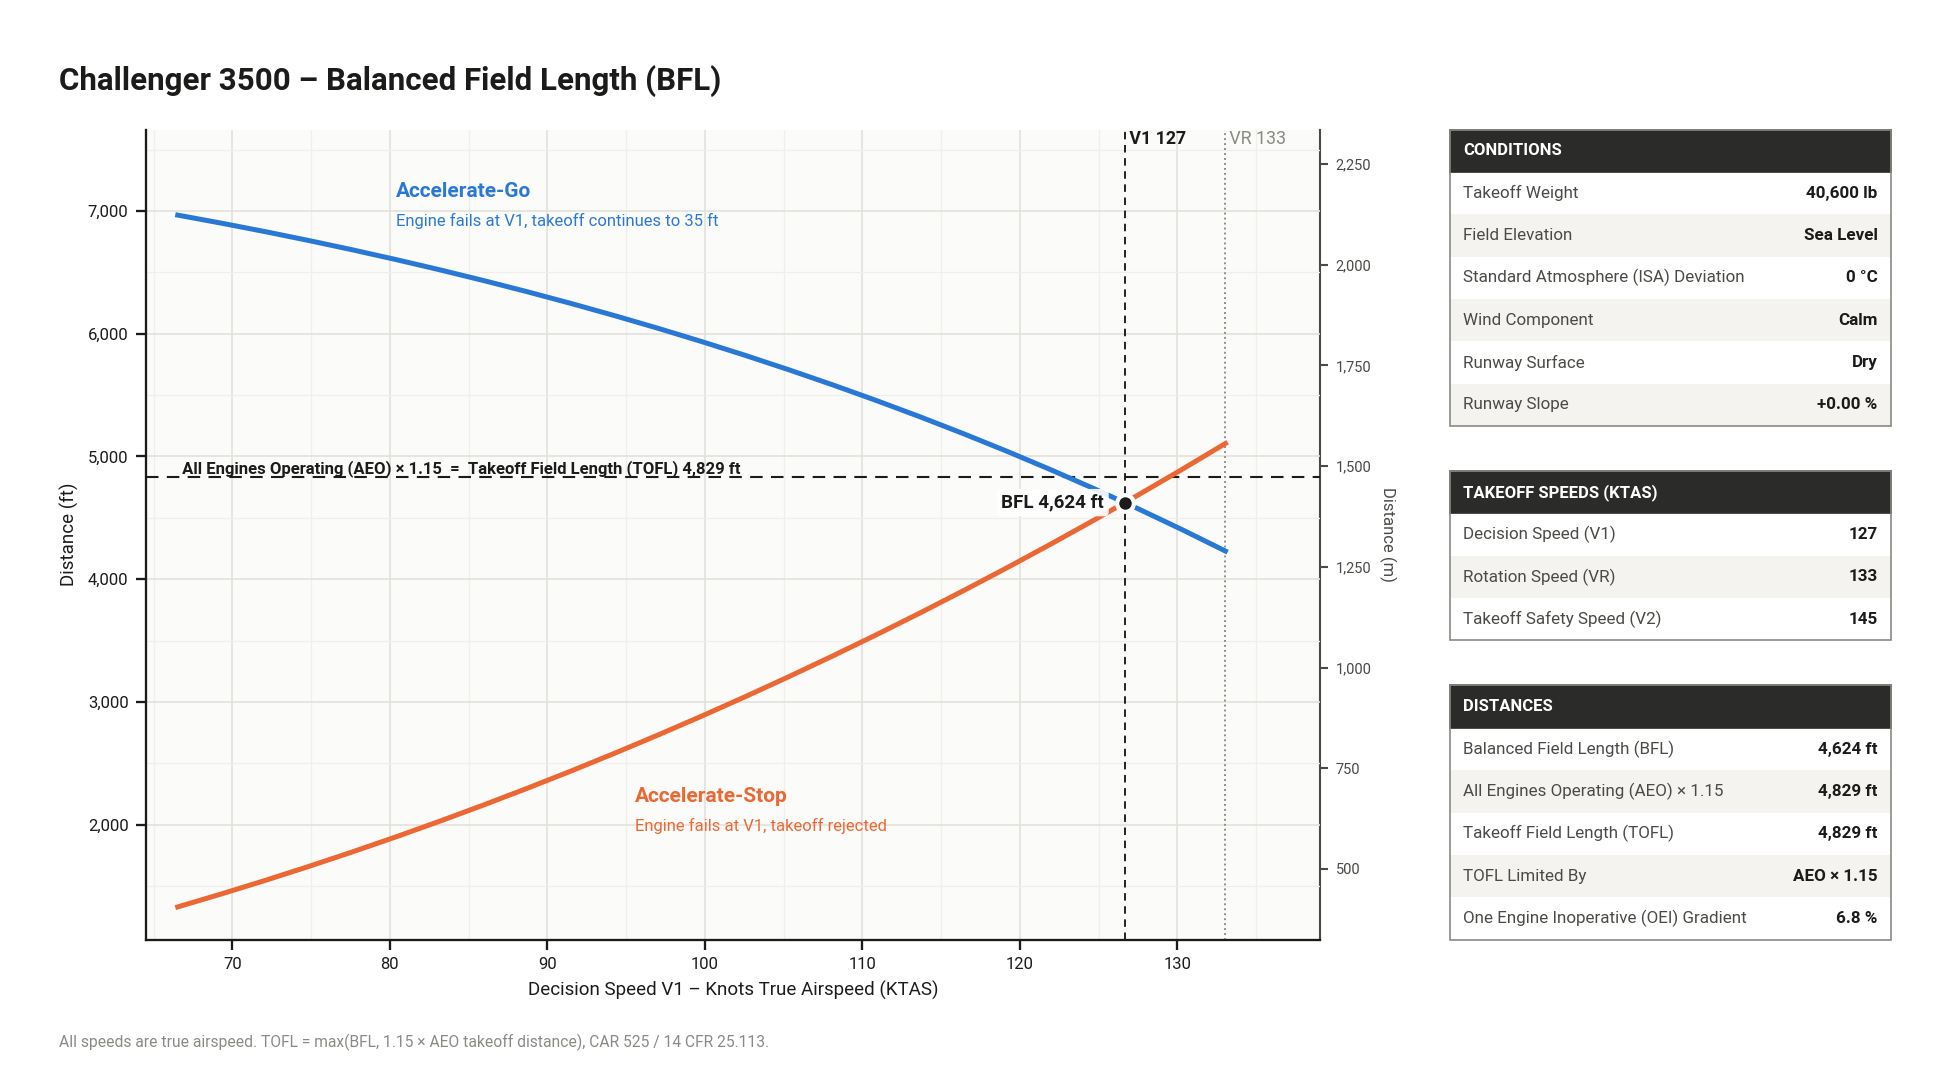
\includegraphics[width=\linewidth]{bfl_Challenger_3500.png}
\begin{enumerate}
\item The horizontal axis is trial $V_1$ in KTAS. The vertical axis is distance.
Each point on a curve is a separate continue-or-stop calculation.
\item The descending accelerate-go curve reflects less OEI acceleration when
failure occurs later. The rising accelerate-stop curve reflects a later rejection.
\item Their crossing gives the balanced decision speed and BFL. Do not choose
$V_1$ beyond $V_R$, even if a plotted extrapolation would appear favourable.
\item Compare the crossing height with the horizontal factored AEO distance.
The larger distance sets TOFL. For this baseline Challenger case, the AEO line
sits above the BFL crossing.
\item A small difference between the two limiting distances means a change in
conditions may change which case governs. Always calculate both.
\end{enumerate}
\selfcheck{If the stop curve moves upward because braking friction decreases,
which way would the crossing normally move? Toward a lower $V_1$, provided the
go curve is unchanged and an intersection still exists within the bounds.}

\topic{Landing distance and landing-distance factors}
\reading{Mair \& Birdsall, Ch.~6 \cite{mair}; Filippone, Sec.~11.7 \cite{filippone}. Operational factors are separate from textbook force balances.}
Landing starts at a 50 ft screen height for both aircraft types:
\begin{align*}
V_{\rm REF}&=1.3V_{S0},\qquad V_{\rm TD}=1.15V_{S0},\\
s_{\rm air}&=\frac{h_{\rm scr}}{\tan3^\circ}
\frac{V_{\rm REF}-V_w}{V_{\rm REF}},\\
s_{\rm free}&=(V_{\rm TD}-V_w)t_{\rm free},\\
\mathrm{LD}&=s_{\rm air}+s_{\rm free}+s_{\rm brake}.
\end{align*}
$t_{\rm free}$ is 2 s for props and 3 s for jets. It represents travel after
touchdown before full braking; the speed is held constant during this segment.
Braking starts at $V_{\rm TD}-V_w$ GS and uses the braking force balance.
The lower touchdown speed approximates speed lost during the flare; the flare
itself is not integrated as a separate flight path.

\textbf{Geometry check:} $50\unit{ft}=15.24\unit m$, so the still-air distance
on a $3^\circ$ approach is $15.24/\tan3^\circ=290.80\unit m$.
With a 60 m/s approach TAS and 5 m/s headwind, the model reduces this to
$290.80(55/60)=266.57$ m.

\textbf{LD versus LDR.} LD is the calculated physical landing distance.
For jets, runway analysis uses:
\[
\mathrm{LDR}_{\rm dry}=\frac{\mathrm{LD}_{\rm dry}}{0.6},\qquad
\mathrm{LDR}_{\rm wet}=1.15\,\mathrm{LDR}_{\rm dry}.
\]
For a dry LD of 800 m, LDR is 1333.33 m dry and 1533.33 m wet.
Dividing by 0.6 increases the requirement; it does not reduce the distance.

\begin{keyidea}
Two different wet effects exist in V7. A wet physical landing uses half the
braking coefficient. The wet jet runway requirement is separately calculated
from the \emph{dry} landing distance and multiplied by 1.15.
Do not apply 1.15 to the wet physical LD and call it the same calculation.
\end{keyidea}
The standalone landing result's LDR field is LD times the aircraft factor for
the supplied conditions. The runway-analysis function performs the separate
dry-baseline recalculation needed for its wet jet requirement. Props have no
LDR factor in this model; their runway check uses unfactored LD.
\selfcheck{If reverse thrust reduces LD, will the default runway report use that
benefit? No. Runway analysis defaults to reverse thrust disabled.}


\theorypage{landing geometry and stopping energy}
\reading{Mair \& Birdsall, Ch.~6 \cite{mair}; Filippone, Sec.~11.7 \cite{filippone}.}
\textbf{Landing distance contains different physical processes.}
The airborne segment loses height, the free-roll segment travels before full
braking, and the braking segment removes ground-frame kinetic energy.
Adding the three distances is reasonable only if the end condition of each
segment matches the start condition of the next.

\textbf{Approach geometry is a triangle approximation.}
At constant descent angle $\gamma$ in still air, the horizontal distance to lose
height $h$ is $s=h/\tan|\gamma|$. For $h=15.24$ m and $|\gamma|=3^\circ$,
$s\approx290.80$ m. A smaller angle requires more horizontal distance.
This simple construction does not independently resolve a flare, touchdown
sink rate or a changing flight path. V7 uses a fixed geometry with a wind
correction; learn that approximation rather than interpreting it as a trajectory
simulation.

\textbf{Delay costs distance even before braking starts.}
At approximately constant touchdown GS, $s_{\rm free}=V_{\rm GS}t_{\rm free}$.
At 30 m/s, each additional second adds about 30 m before the braking calculation.
Then a simplified constant-deceleration estimate gives $s_{\rm brake}=V_0^2/(2b)$.
This explains why touchdown speed and delay can matter as much as braking strength.
In V7, forces change during braking, so integration replaces that simple estimate.

\textbf{Separate a physical prediction from an operating allowance.}
Physical LD estimates the distance taken by the modeled landing. Factored LDR
is a requirement used for a runway comparison. A multiplier changes the required
distance; it does not change the simulated force balance or add real brake force.
The project's dry and wet factors belong to this second category.

Wetness appears in two distinct ways: V7 can reduce the braking coefficient in
a physical wet landing, and its jet runway analysis can apply a wet multiplier
to the dry-based factored requirement. Combining these without following the
specified calculation would answer a different question.

\begin{keyidea}
\textbf{Explain aloud:} the landing model joins a geometry estimate, a delay
estimate and a braking trajectory. Operational factors are applied to a defined
baseline after the physical calculation; they are not extra forces.
\end{keyidea}

\topic{Runway checks, margins and sensitivity}
\reading{Ojha \cite{ojha} and Filippone, Ch.~9 \cite{filippone}, for performance context. The margin definitions and scenario choices below follow V7.}
\par
\begin{tabularx}{\linewidth}{@{}lX@{}}\toprule
Abbreviation & Available distance\\\midrule
TORA & Takeoff Run Available: ground run.\\
TODA & Takeoff Distance Available: takeoff distance including permitted clearway.\\
ASDA & Accelerate-Stop Distance Available: stopping distance including permitted stopway.\\
LDA & Landing Distance Available.\\\bottomrule
\end{tabularx}
For built-in runways, V7 simplifies TORA = TODA = ASDA = runway length and
LDA = runway length minus the displaced threshold. It does not model actual
clearway/stopway declarations independently for those defaults.
\begin{align*}
\text{Twin takeoff:}&\quad\mathrm{TOFL}\le\mathrm{TODA},\quad\mathrm{ASD}\le\mathrm{ASDA},\\
\text{Single takeoff:}&\quad\mathrm{TOD}\le\mathrm{TODA},\quad s_{\rm ground}\le\mathrm{TORA},\\
\text{Jet landing:}&\quad\mathrm{LDR}\le\mathrm{LDA},\\
\text{Prop landing:}&\quad\mathrm{LD}\le\mathrm{LDA}.
\end{align*}
\[
\mathrm{margin}=\mathrm{available}-\mathrm{required}.
\]
A zero margin passes the implemented comparison. A negative margin fails it.
Passing these checks does not prove obstacle clearance, brake-energy compliance,
OEI second-segment climb compliance or an acceptable crosswind.

\textbf{KICT 01L example.} Challenger at MTOW/MLW, OAT $30^\circ$C, reported
wind $020^\circ$/10 kt, dry runway: ISA deviation is +\val{kictisa}$^\circ$C and
performance headwind is \val{kictwind} kt. Available distances are 10302 ft.
TOFL is \val{kicttofl} ft; ASD is \val{kictasd} ft; LDR is \val{kictldr} ft.
The landing margin is therefore \val{kictmargin} ft.

\textbf{Sensitivity calculation:}
\[
\Delta_{\%}=100\left(\frac{s}{s_{\rm baseline}}-1\right).
\]
Changing distance from 1500 to 1800 m gives +20\%; changing it to 1200 m gives
$-20\%$. The sweeps change one input at a time; takeoff weight is a percentage
of MTOW, landing weight a percentage of MLW. A sweep is not a combined hot/high,
heavy, tailwind worst-case assessment.
\selfcheck{Why can two aircraft have the same percentage weight setting but different
masses? Their MTOW and MLW are different reference values.}

\topic{A complete C172 calculation to explain aloud}
\textbf{Inputs:} sea level, ISA, calm wind, dry level runway, MTOW = MLW = 2550 lb;
$S=16.2$ m$^2$, $C_{L,\max,TO}=1.5$, $C_{L,\max,LDG}=2.0$,
$C_{L,\rm gnd}=0.4$, $C_{D_0}=0.032$, $k=0.045$,
$\mu_{\rm roll}=0.04$, $\mu_{\rm brake}=0.40$.
\begin{enumerate}
\item Convert mass: $m=\val{mass}$ kg and $W=\val{weight}$ N.
\item Calculate the atmosphere: $\rho=\val{rho}$ kg/m$^3$ and $a=\val{sound}$ m/s.
The density is slightly different from exactly 1.225 because the stored gas
constant and sea-level density reference are rounded independently.
\item Derive speeds: $V_{S1}=\val{vs}$ m/s, $V_R=\val{vr}$ m/s,
$V_2=\val{vtwo}$ m/s.
\item At $V_R$, calculate $q=\val{q}$ Pa, $L=\val{lift}$ N,
$D=\val{drag}$ N and $T=\val{thrust}$ N.
\item Rolling friction is \val{friction} N, giving instantaneous acceleration
\val{accel} m/s$^2$. This is one point on the trajectory, not the average.
\item Integrate acceleration to $V_R$, then add \val{rot} m for rotation.
Total ground distance is \val{roll} m, including rotation; total ground time
is \val{rolltime} s.
\item Use excess thrust at $V_2$ to obtain a climb gradient of \val{grad}\%.
The transition/climb calculation adds \val{air} m to the 50 ft screen.
\item TOD is $\val{roll}+\val{air}=\val{tod}$ m, or \val{todft} ft
(the displayed rounded components may differ slightly in their last digit).
\item For landing, use $V_{\rm REF}=\val{vref}$ m/s and
$V_{\rm TD}=\val{vtd}$ m/s. The air, free-roll and braking distances are
\val{ldair}, \val{free} and \val{brake} m.
\item LD is \val{ld} m, or \val{ldft} ft. No jet LDR factor is applied.
\end{enumerate}
\begin{keyidea}
You should be able to explain where every number in this chain comes from.
The ground-roll and braking totals require integration; they cannot be reproduced
exactly by substituting one average acceleration into a closed-form equation.
\end{keyidea}

\topic{What changes what, and why}
\par
\begin{tabularx}{\linewidth}{@{}p{0.22\linewidth}X@{}}\toprule
Change & Main reasoning to explain\\\midrule
Higher pressure altitude & Density usually falls; stall and scheduled TAS rise.
Engine thrust/power may fall. More GS and less excess force tend to increase distance.\\
Higher OAT & Density falls at fixed pressure altitude. Engine response depends
on the turbocharging or flat-rating approximation.\\
Higher mass & Weight and required lift rise; stall speed rises as $\sqrt W$.
There is more kinetic energy at a given GS and less acceleration for a given net force.\\
Headwind & Target TAS is reached at lower GS. The ground-distance and airborne
wind corrections generally reduce the required distance.\\
Tailwind & Higher GS is needed for the same TAS; distance generally increases.
The runway-analysis factor magnifies the input penalty.\\
Uphill slope & Reduces acceleration, assists braking. Downhill reverses those effects.\\
Wet runway & Weaker tyre braking increases stopping distance. V7 does not
implement the full wet takeoff treatment.\\
Ground spoilers & Lower lift puts more weight on the wheels and increases braking force.\\
Higher $C_{L,\max}$ & Lowers stall speed and the scheduled speeds. It does not
by itself specify the real drag cost of a flap change.\\\bottomrule
\end{tabularx}
\textbf{Calibration versus validation.} Calibration adjusts an input to reproduce
a chosen target. V7 calibrates Challenger takeoff $C_{L,\max}$ to TOFL and SR22T
static thrust to takeoff ground roll. Matching those targets is not independent
validation. Landing distances or other conditions not used for tuning provide
separate comparisons, with their own data uncertainty.

\textbf{Know the main omissions:} QNH correction; IAS/CAS conversion; a full
engine deck; failed-engine drag; VMCG/VMU schedules; second-segment OEI/WAT limits;
brake-energy limits; complete wet-runway certification; verified declared runway
distances. These explain why a plausible numerical result can still be incomplete.
\selfcheck{What would you improve first? State a specific missing effect, the data
needed to model it, and an independent comparison that would test the change.}


\theorypage{what a sensitivity result can and cannot prove}
\reading{Performance context: Ojha \cite{ojha}; the distinctions below apply to the V7 scenario calculations.}
\textbf{A calculation answers a conditional question.}
A model output means: with these inputs, coefficients and assumptions, the
equations predict this result. Changing one input while holding others fixed
shows a conditional sensitivity. It does not isolate every effect that would
change together in a real aircraft operation.

\textbf{Separate absolute change from percentage change.}
For a baseline $s_0$ and changed case $s_1$,
\[
\Delta s=s_1-s_0,\qquad
\Delta s_{\%}=100\frac{s_1-s_0}{s_0}.
\]
An additional 100 m is a 20\% increase from 500 m but only 5\% from 2000 m.
Report the reference condition with every percentage. A sweep over many inputs
is not equivalent to a local derivative at one condition.

\textbf{Use a small perturbation to estimate local sensitivity.}
For an input $x$ and a small increment $\delta x$, a central difference is
\[
\frac{\partial s}{\partial x}\approx
\frac{s(x+\delta x)-s(x-\delta x)}{2\delta x}.
\]
The units matter: metres per kilogram differs from metres per degree Celsius.
Very small perturbations can expose numerical noise; large ones average over
nonlinear changes. A switch between BFL-controlled and AEO-controlled TOFL can
also create a corner where a single smooth derivative is misleading.
This derivative is an optional analysis technique, not a claim that V7's
existing percentage sweep uses it.

\textbf{Calibration does not supply independent evidence.}
Adjusting static thrust to match one measured roll can make that example agree
by construction. Other parameter combinations might match it too. Assess the
model against conditions not used for tuning: different weights, temperatures,
altitudes or speeds. Otherwise, you cannot tell whether the fitted parameter
captures the intended physics or compensates for another missing effect.

\textbf{A runway margin is only as strong as the requirement behind it.}
Margin is available distance minus required distance. Positive margin means the
modeled comparison passes. It does not account for omitted obstacles, incorrect
inputs or unmodeled operational constraints. Greater numerical precision cannot
remove uncertainty in friction, thrust or maximum lift coefficient.

\begin{keyidea}
\textbf{Explain aloud:} verification asks whether the equations were solved
correctly; validation asks whether those equations describe the intended physical
case well enough. Calibration fits parameters; sensitivity measures response.
These are related tasks, but none substitutes for the others.
\end{keyidea}

\topic{Practice questions: try these without the answers}
Use $g_0=9.80665$ m/s$^2$; round only at the end.
\begin{enumerate}[label=\textbf{\arabic*.}]
\item Convert 100 kt to m/s and 5000 ft to m. Convert 3000 lb to mass and weight in SI.
\item At 1500 m pressure altitude and OAT $25^\circ$C, find standard temperature
in K and $^\circ$C, ISA deviation and actual temperature in K.
\item For $p=90000$ Pa and $\Theta=300$ K, calculate density and $\sigma$.
\item Wind is from $060^\circ$ at 20 kt on a runway heading $030^\circ$.
Find headwind, crosswind and performance headwind.
\item With $\rho=1.1$ kg/m$^3$, $V=50$ m/s, $S=20$ m$^2$ and $C_L=0.6$,
find $q$ and lift. With $C_{D_0}=0.03$ and $k=0.05$, find drag.
\item For $W=20000$ N, $\rho=1.1$, $S=20$ and $C_{L,\max}=1.6$,
calculate $V_{S1}$, $V_R$ and $V_2$ in m/s.
\item If weight rises by 21\% with density and $C_{L,\max}$ unchanged,
what is the percentage increase in stall speed?
\item For $P=200000$ W, $\eta_p=0.75$, $V=30$ m/s,
$T_{\rm SLS}=4000$ N and $\sigma_P=1$, find propeller thrust with all engines.
\item A twin has AEO thrust 50000 N, drag 20000 N and weight 200000 N.
Compare AEO and OEI climb gradients using the project's steady-climb relations.
\item An aircraft reaches 40 m/s GS from rest at a constant 2 m/s$^2$.
Find time and distance. Explain why this is only a check for the real model.
\item At $V_R=60$ m/s TAS with 5 m/s headwind and a 3 s rotation,
what rotation distance is added?
\item Let $V_{\rm TR}=60$ m/s, $n=1.2$ and $\gamma=0.10$ rad.
Find $R_{\rm TR}$ and $h_{\rm TR}$. Does a 10 m screen lie within the arc?
\item BFL is 1400 m and AEO TOD is 1300 m. Find TOFL and the limiting case.
\item Dry jet LD is 900 m and LDA is 1700 m. Find dry and wet LDR and margins.
\item Distance rises from 1600 to 1840 m. Find the percentage change.
If TOFL passes TODA but ASD exceeds ASDA, does takeoff pass?
\end{enumerate}

\topic{Worked answers}
\begin{enumerate}[label=\textbf{\arabic*.}]
\item $100(1852/3600)=51.4444$ m/s; $5000(0.3048)=1524$ m.
Mass $=3000(0.45359237)=1360.7771$ kg; weight $=13344.6648$ N.
\item $\Theta_{\rm std}=288.15-0.0065(1500)=278.40$ K, or $5.25^\circ$C.
ISA deviation $=25-5.25=19.75^\circ$C. Actual temperature $=298.15$ K.
\item $\rho=90000/(287.05\times300)=1.0451$ kg/m$^3$;
$\sigma=\rho/1.225=0.8532$.
\item Heading difference $=30^\circ$.
Headwind $=17.3205$ kt, crosswind $=10$ kt from the right;
performance headwind $=8.6603$ kt.
\item $q=0.5(1.1)(50)^2=1375$ Pa; $L=1375(20)(0.6)=16500$ N.
$C_D=0.03+0.05(0.6)^2=0.048$; $D=1320$ N.
\item $V_{S1}=\sqrt{40000/(1.1\times20\times1.6)}=33.7100$ m/s;
$V_R=37.0810$ m/s; $V_2=40.4520$ m/s.
\item Speed factor $=\sqrt{1.21}=1.10$: a 10\% increase.
\item Power-based thrust $=0.75(200000)/30=5000$ N.
Static cap $=4000$ N, so thrust is 4000 N.
\item AEO: $\sin\gamma=(50000-20000)/200000=0.15$;
gradient $=100\tan(\arcsin0.15)=15.17\%$.
OEI thrust $=25000$ N, giving $\sin\gamma=0.025$ and gradient $=2.501\%$.
Half the thrust leaves only one-sixth of the original excess thrust.
\item $t=40/2=20$ s; $s=40^2/(2\times2)=400$ m.
Actual thrust, drag and friction vary during the ground roll.
\item $s_{\rm rot}=(60-5)(3)=165$ m.
\item $R_{\rm TR}=60^2/[9.80665(0.2)]=1835.49$ m;
$h_{\rm TR}=1835.49(1-\cos0.10)=9.17$ m.
The 10 m screen is above the completed arc, so add a short straight-climb segment.
\item $1.15(1300)=1495$ m, larger than BFL. TOFL = 1495 m, AEO-limited.
\item Dry LDR $=900/0.6=1500$ m, margin $=+200$ m.
Wet LDR $=1.15(1500)=1725$ m, margin $=-25$ m: wet requirement fails.
\item $100(1840/1600-1)=15\%$. The takeoff check fails if ASD exceeds ASDA,
even if TOFL fits within TODA.
\end{enumerate}

\topic{Questions you should be able to answer aloud}
\begin{enumerate}
\item \textbf{Why use TAS for forces and GS for distance?} Air loads depend on
relative airflow; runway travel depends on motion relative to the ground.
\item \textbf{Why does hot-and-high operation need more runway?} Lower density
raises the scheduled TAS and can reduce propulsion. The size of each effect depends
on the engine model and the particular case.
\item \textbf{Why not use a single acceleration value?} The force balance changes
with speed, especially thrust, aerodynamic loads and wheel friction.
\item \textbf{Why can spoilers improve stopping?} They reduce lift, increase wheel
load and increase the available tyre braking force in the model.
\item \textbf{What is BFL?} The go/stop distance at their crossing, when a valid
crossing exists within the selected decision-speed bounds.
\item \textbf{Why might TOFL exceed BFL?} The factored AEO distance may be larger.
\item \textbf{What makes a root-finding method different from an integrator?}
Integration predicts a trajectory for given conditions. Root finding changes $V_1$
until two integrated distance outcomes agree.
\item \textbf{What does a calibration match prove?} That a selected parameter can
reproduce that target, not that the complete model is independently validated.
\item \textbf{Why are the fixed speed ratios limited?} Real schedules also depend
on configuration, control speeds, certification constraints and manufacturer data.
\item \textbf{Which wet landing distance is factored?} Runway analysis uses the
dry jet LD for its LDR factor and wet multiplier, separately from wet physical braking.
\item \textbf{What does a positive runway margin prove?} Only that the specified
model requirement fits the supplied available distance under the selected assumptions.
\item \textbf{How would you test an improvement?} Use data not used to tune it,
compare several operating conditions, and separate numerical error from model error.
\end{enumerate}
\begin{keyidea}
You are ready to explain the project when you can reconstruct the C172 example,
explain the BFL chart, solve the practice set and identify the main limitations
without reading a prepared script.
\end{keyidea}

\topic{Compact equation checklist}
\begin{align*}
W&=mg_0,&q&=\tfrac12\rho V^2,\\
\rho&=p/(R\Theta),&a&=\sqrt{1.4R\Theta},\\
L&=qSC_L,&D&=qS(C_{D_0}+kC_L^2),\\
V_S&=\sqrt{2W/(\rho SC_{L,\max})},&V_{\rm GS}&=V_{\rm TAS}-V_w,\\
\dot V_{\rm GS,accel}&=(T-D-\mu_{\rm roll}N-W\sin\theta)/m,\\
\dot V_{\rm GS,brake}&=-(D+\mu_{\rm brake}N+T_{\rm rev}+W\sin\theta)/m,\\
\sin\gamma&=(T-D)/W,&G_{\%}&=100\tan\gamma,\\
R_{\rm TR}&=V_{\rm TR}^2/[g_0(n-1)],&h_{\rm TR}&=R_{\rm TR}(1-\cos\gamma),\\
\mathrm{TOD}&=s_{\rm roll}+s_{\rm rot}+s_{\rm air},\\
\mathrm{TOFL}&=\max(\mathrm{BFL},1.15\mathrm{TOD}_{\rm AEO}),\\
\mathrm{LD}&=s_{\rm air}+s_{\rm free}+s_{\rm brake},\\
\mathrm{LDR}_{\rm dry}&=\mathrm{LD}_{\rm dry}/0.6,&
\mathrm{LDR}_{\rm wet}&=1.15\mathrm{LDR}_{\rm dry}.
\end{align*}
Here $N=\max(W-L,0)$ is the project's wheel-load approximation. Keep the detailed
piecewise propulsion, wind and transition equations from the earlier sections.

\textbf{Source of the project-specific equations and values.}
The current V7 files \texttt{atmosphere.py}, \texttt{aircraft.py},
\texttt{segments.py}, \texttt{takeoff.py}, \texttt{bfl.py}, \texttt{landing.py},
\texttt{airports.py}, \texttt{runway\_analysis.py}, \texttt{sensitivity.py} and
\texttt{units.py}. The methodology report and \texttt{REFERENCES.md} give the
project's textbook and regulatory references. The factors here describe the
implementation; this guide is not a current regulatory compliance review.

\textbf{Additional explanations checked for this guide:}
\begin{itemize}
\item NASA Glenn, \href{https://www1.grc.nasa.gov/beginners-guide-to-aeronautics/lift-equation-2/}{Lift Equation} and
\href{https://www1.grc.nasa.gov/beginners-guide-to-aeronautics/drag-equation/}{Drag Equation}: definitions of aerodynamic force and coefficients.
\item NASA Glenn, \href{https://www1.grc.nasa.gov/beginners-guide-to-aeronautics/induced-drag-coefficient/}{Induced Drag Coefficient}: finite-wing interpretation of $k$.
\item NASA Glenn, \href{https://www1.grc.nasa.gov/beginners-guide-to-aeronautics/earth-atmosphere-equation-metric/}{Earth Atmosphere Equation}: atmosphere-model background. Its curve-fit constants differ from V7; use V7's constants for matching calculations.
\end{itemize}

\topic{Textbook reading map}
Use the topic citations to connect a calculation to its physical background.
For a first pass, read Mair \& Birdsall alongside the force balances. Use
Filippone for a more detailed treatment of field performance and engine models.

\begin{tabularx}{\linewidth}{@{}p{0.23\linewidth}XX@{}}
\toprule
Topic & Mair \& Birdsall \cite{mair} & Filippone \cite{filippone}\\\midrule
Aerodynamics & Chs.~1--3 & Ch.~4\\
Atmosphere and speeds & Ch.~2 (flight theory) & Secs.~8.1--8.2\\
Propulsion & Ch.~5 & Chs.~5--6\\
Ground run & Ch.~6 & Secs.~9.2--9.3\\
OEI and stopping & Ch.~6 & Sec.~9.4\\
Climb & Ch.~4 & Ch.~10\\
Landing & Ch.~6 & Sec.~11.7\\\bottomrule
\end{tabularx}

\textbf{Other useful textbooks in the project bibliography.}
Anderson's two books \cite{anderson-performance,anderson-flight} support the
fundamentals. Raymer \cite{raymer} and Torenbeek \cite{torenbeek} put performance
estimates in the wider aircraft-design process. Gudmundsson \cite{gudmundsson}
is especially relevant to general aviation; Ojha \cite{ojha} provides another
flight-performance treatment. These are book-level recommendations, without
claims about specific pages or identical implementations.

\begin{keyidea}
\textbf{Keep the source categories separate.}
Newton's law and aerodynamic definitions supply the physical framework.
The code supplies the numerical constants, piecewise engine fits, fixed speed
ratios, wet-braking reduction and integration settings used in these examples.
Regulations supply requirements in their stated scope; a simplified implementation
of a factor does not reproduce an entire certification or operating rule.
\end{keyidea}

\textbf{Checking the reading pointers.}
The publisher's \href{https://www.cambridge.org/core/books/abs/aircraft-performance/index/0715423089460781606F4D741A91D1D5}{contents listing for Mair \& Birdsall}
and \href{https://assets.cambridge.org/97811070/24007/frontmatter/9781107024007_frontmatter.pdf}{front matter for Filippone}
identify the chapters and sections above. These checks establish where to read,
not a page-by-page verification of the textbooks' equations.

\textbf{Regulatory reading recorded by V7.}
The project cites 14 CFR 25.105, 25.109 and 25.113 for takeoff context and
\href{https://www.ecfr.gov/current/title-14/chapter-I/subchapter-G/part-121/subpart-I/section-121.195}{14 CFR 121.195}
for landing limitations. Consult the applicable rule and aircraft data before
interpreting these factors outside the educational model.

\clearpage
\phantomsection
\addcontentsline{toc}{section}{References}
\renewcommand{\refname}{References}
\begin{thebibliography}{10}
\setlength{\itemsep}{9pt}
\bibitem{anderson-performance}
Anderson, John D., Jr. \emph{Aircraft Performance and Design}.
McGraw-Hill, 1999.
\bibitem{anderson-flight}
Anderson, John D., Jr. \emph{Introduction to Flight}. 8th ed.,
McGraw-Hill Education, 2016.
\bibitem{mair}
Mair, W. Austyn, and David L. Birdsall. \emph{Aircraft Performance}.
Cambridge University Press, 1992.
\href{https://doi.org/10.1017/CBO9780511607134}{doi:10.1017/CBO9780511607134}.
\bibitem{filippone}
Filippone, Antonio. \emph{Advanced Aircraft Flight Performance}.
Cambridge University Press, 2012 (print edition).
\href{https://doi.org/10.1017/CBO9781139161893}{doi:10.1017/CBO9781139161893}.
\bibitem{raymer}
Raymer, Daniel P. \emph{Aircraft Design: A Conceptual Approach}.
6th ed., American Institute of Aeronautics and Astronautics, 2018.
\bibitem{torenbeek}
Torenbeek, Egbert. \emph{Synthesis of Subsonic Airplane Design}.
Delft University Press / Kluwer Academic Publishers, 1982.
\href{https://doi.org/10.1007/978-94-017-3202-4}{doi:10.1007/978-94-017-3202-4}.
\bibitem{gudmundsson}
Gudmundsson, Snorri. \emph{General Aviation Aircraft Design:
Applied Methods and Procedures}. 1st ed., Butterworth-Heinemann, 2014.
\bibitem{ojha}
Ojha, S. K. \emph{Flight Performance of Aircraft}.
American Institute of Aeronautics and Astronautics, 1995.
\bibitem{scipy-ivp}
SciPy developers. \texttt{scipy.integrate.solve\_ivp}, API documentation.
\href{https://docs.scipy.org/doc/scipy/reference/generated/scipy.integrate.solve_ivp.html}{Solver methods, tolerances and events}. Accessed 4 November 2026.
\bibitem{scipy-brent}
SciPy developers. \texttt{scipy.optimize.brentq}, API documentation.
\href{https://docs.scipy.org/doc/scipy/reference/generated/scipy.optimize.brentq.html}{Bracketed scalar root finding}. Accessed 4 November 2026.
\end{thebibliography}

\end{document}
